\documentclass{article}
\usepackage{tikz}
\usetikzlibrary{calc,shapes,decorations.markings}
\usepgflibrary{shapes.geometric}

% Syntax: \Cylinder{<x-coordinate>}{<y-coordinate>}{<name>}{<shownName>}
\newcommand\drawOsdCylinder[4]{%
\tikzset{Cylin/.style={cylinder, shape border rotate = 90, draw, cylinder uses custom fill,
cylinder end fill = blue!20, cylinder body fill = blue!20, minimum height =2cm,
minimum width = 1.5cm, opacity = 1, aspect = 0.5}}
\node[Cylin] (#3) at (#1,#2) {#4};
}

\newcommand\drawMdsCube[2] {
\coordinate(p) at (#1,#2);
\draw[fill = red!20] ($ (p) + (-1,0.5) $) -- ($ (p) + (-0.75,0.75) $) -- ($ (p) + (1.25, 0.75)$) -- ($ (p) + (1, 0.5) $);
\draw[fill = red!20] ($ (p) + (1.25, 0.75)$) -- ($ (p) + (1.25, -0.25) $) -- ($ (p) + (1, -0.5) $) -- ($ (p) + (1, 0.5) $);
\node[rectangle, draw, fill = red!20, minimum width=2cm, minimum height=1cm] () at (#1,#2) {MDS};
}

\newcommand\drawClientCircle[2] {
\coordinate(p) at (#1, #2);
\node[circle, draw, fill = green!20, minimum width=2cm] at ($ (p)+(0.2,0.2) $) {};
\node[circle, draw, fill = green!20, minimum width=2cm] at ($ (p)+(0.1,0.1) $) {};
\node[circle, draw, fill = green!20, minimum width=2cm] at (p) {CLIENTS};
}

\newcommand\drawMonitorDiamond[2] {
\node[diamond, draw, fill = yellow!20, minimum width=1.5cm, minimum height =
1.5cm] () at (#1, #2) {MONITOR};
}
\newcommand\drawArch{
\begin{figure}[!h]
	\begin{center}
		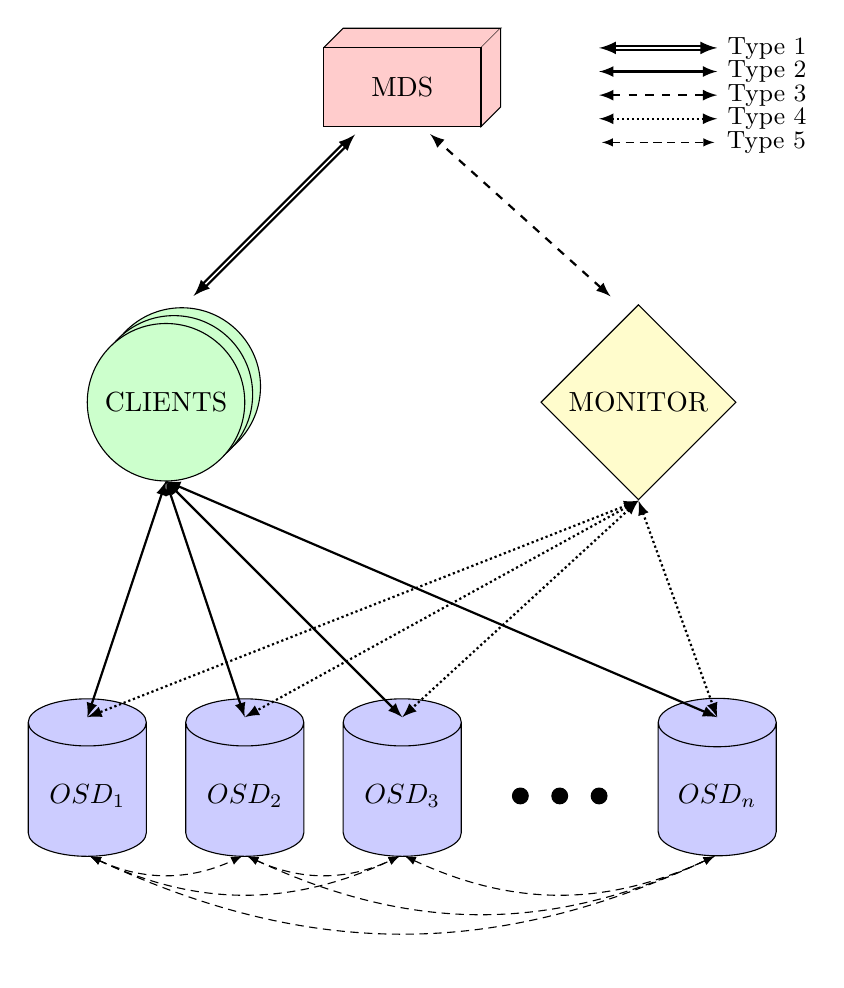
\begin{tikzpicture}[
			t5/.style={thin,<->, densely dashed,bend right=25, shorten >=1pt,shorten <=1pt,>=latex},
			t1/.style={thick,<->,double, shorten >=4pt,shorten <=4pt,>=latex},
			tt1/.style={thick,<->,double, shorten >=0pt,shorten <=0pt,>=latex},
			t2/.style={thick,<->,shorten >=0pt,shorten <=0pt,>=latex},
			t3/.style={thick,<->, dashed, shorten >=4pt,shorten <=4pt,>=latex},
			tt3/.style={thick,<->, dashed, shorten >=0pt,shorten <=0pt,>=latex},
			t4/.style={thick,densely dotted,<->,shorten >=0pt,shorten <=0pt,>=latex}]

			%\whitebodyCylinder{0}{0}{}
			%\draw[help lines] (0,0) grid (10, 10);
			% drawing OSDs
			\drawOsdCylinder{1}{0}{osd1}{$OSD_1$} \drawOsdCylinder{3}{0}{osd2}{$OSD_2$}
			\drawOsdCylinder{5}{0}{osd3}{$OSD_3$}
			\filldraw[black] (6.5,0) circle(0.1);
			\filldraw[black] (7,0) circle(0.1);
			\filldraw[black] (7.5,0) circle(0.1);
			\drawOsdCylinder{9}{0}{osdn}{$OSD_n$}

			% drawing MDS
			\drawMdsCube{5}{9}

			% drawing Clients
			\drawClientCircle{2}{5}

			% drawing Monitor
			\drawMonitorDiamond{8}{5}

			% drawing arrow
			\draw[t1] (2.25, 6.25) -- (4.5, 8.5) {};

			\draw[t2] (2,4) -- (1, 1) {};
			\draw[t2] (2,4) -- (3, 1) {};
			\draw[t2] (2,4) -- (5, 1) {};
			\draw[t2] (2,4) -- (9, 1) {};

			\draw[t3] (7.75,6.25) -- (5.25,8.5) {};

			\draw[t4] (8,3.75) -- (1,1) {};
			\draw[t4] (8,3.75) -- (3,1) {};
			\draw[t4] (8,3.75) -- (5,1) {};
			\draw[t4] (8,3.75) -- (9,1) {};

			% sample arrow
			\draw[tt1] (7.5,9.5) -- (9,9.5) node[right, right] {\small{Type 1}};
			\draw[t2] (7.5,9.2) -- (9,9.2) node[right, right] {\small{Type 2}};
			\draw[tt3] (7.5,8.9) -- (9,8.9) node[right, right] {\small{Type 3}};
			\draw[t4] (7.5,8.6) -- (9,8.6) node[right, right] {\small{Type 4}};
			\draw[t5] (7.5,8.3) -- (9,8.3) node[right, right] {\small{Type 5}};

			\draw[t5] (1,-0.75) to (3, -0.75) {};
			\draw[t5] (1,-0.75) to (5, -0.75) {};
			\draw[t5] (1,-0.75) to (9, -0.75) {};
			\draw[t5] (3,-0.75) to (5, -0.75) {};
			\draw[t5] (3,-0.75) to (9, -0.75) {};
			\draw[t5] (5,-0.75) to (9, -0.75) {};

		\end{tikzpicture}
	\end{center}
	\label{arch}
	\caption{Architecture of NCVFS}
\end{figure}
}


\title{Network Coding Video File System}
\author{Documentation v0.2}
\date{\today}

\usepackage{natbib}
\usepackage{graphicx}
\usepackage{setspace}
\usepackage{url}
\usepackage[utf8]{inputenc}
\doublespacing

\def\osd{\texttt{OSD} }
\def\osds{\texttt{OSDs} }
\def\mds{\texttt{MDS} }
\def\fuse{\texttt{FUSE} }
\def\client{\texttt{CLIENT} }
\def\clients{\texttt{CLIENTs} }
\def\monitor{\texttt{MONITOR} }

\begin{document}

\maketitle

\section{Introduction}
\textit{Cloud Storage} has been playing an increasingly significant
role in data storage for enterprises and individuals lately.
For instance, \textit{Amazon S3} and \textit{Windows Azure} are two successful
clould storage systems in real-life business.
To achieve high data availability, a \textit{distributed storage system} 
is the underlying system architecture adopted by clould storage systems,
as it provides a reliable platform for storing a
massive amount of data over a set of distributed storage nodes over a 
network. Current distributed storage systems mainly apply 
\textit{data replication} to maintain data
reliability, such as \textit{HDFS} and \textit{GFS}. 
Each piece of data in the system is replicated several 
times and each replica is distributed to different storage nodes. 
The \textit{replication factor} determines the number of times each 
piece of data being replicated and therefore, 
data availability is positively related with
the \textit{replication factor} of the entire system. 

However, one major drawback of data replication is that it requires 
relatively large amount of storage resources in order to achieve  
high availability, compared with employing \textit{erasure coding} on
data. 
Moreover, given the similar network bandwith and storage resources, 
systems employing erasure coding has better availability and durability
than systems employing data replication~\cite{Weatherspoon:2002:ECV:646334.687814}.
Under such circumstance, cloud storage systems like \textit{Windows Azure}
and 
\textit{Hadoop Distributed File System} are switching their storage scheme
from replication to erasure coding~\cite{Huang:2012:ECW:2342821.2342823,
hdfs:raid}.

Data repliacation may not fully utilize the parallelism benefit of
distributed storage system if the size of data to be replicated is large. 
Hence, previous researches~\cite{Mesnier03object-basedstorage,Wang04obfs:a} 
have proposed \textit{object-based} storage
systems to handle this issue. In general, an 
object-based storage system splits 
each file to be stored into equal size pieces called \textit{objects}, 
and assigns different storage
nodes to perform replication or coding on the objects. It can
be found that object-based storage systems benefit more than 
file-based storage
systems in a distributed environment due to the parallel processing.

The above-mentioned issues motivate us to design a brand new distributed 
storage
system which could combine the advantages of both erasure coding and 
object-based
stroage techniques to achieve high availability and performance. 
% TODO: May need something between network coding and erasure coding
Hence, in this paper, we present our design and implementation of a 
network-coding-based distributed video file system, called NCVFS.  
The main features of NCVFS are summarized as follows:

\begin{itemize}

	\item NCVFS is an object-based distributed file system targeting 
		large video files. It supports general read and write operations 
		in a distributed storage setting and optimizes the read operation 
		based on the write-once-read-many feature of video files.

	\item NCVFS is not limited by erasure coding storage schemes, but can 
		be extended	to other coding schemes like network coding. 
		Moreover, since NCVFS adopts object-based storage, it enables 
		multiple coding schemes performed on a single file without 
		changing the entire system logic.

	\item NCVFS excludes metadata management from the critical path for the
		read/write process to eliminate the bottleneck of metadata operations 
		and utilizes a centralized monitor to balance the workload of each
		storage node.

	\item NCVFS implements a distributed light-weight recovery scheme to 
		handle storage node failures. In brief, once a recovery process
		is triggered for a particular storage node, NCVFS delays the
		process for a few minutes to confirm the storage node is
		dead permanently. Such delay saves the recovery operations
		for temporary failures like network partition while data on 
		the failed node can still be accessed via degraded read during
		the delay.

\end{itemize}

\section{Revision History}
Version 0.2 (11 September 2012)

\section{System Overview}

\subsection{Architecture}
NCVFS is an object-based distributed file system and is composed of 
four components: metadata storage,
object storage, clients and monitors. A single metadata server (\texttt{MDS}) 
is designed for NCVFS for 
storing all file metadata as well as managing operations on file 
metadata. On top of that, 
NCVFS contains multiple object stroage devices (\texttt{OSDs}) 
and each \osd stores file data objects with
network coding. One
key point of this architecture is that the \mds is not on the 
critical path when clients want to 
read or write files,as the \mds is contacted by clients first 
before clients operate with \osds. Such
design eliminates the bottleneck on the metadata side and enables 
parallel jobs on the object
storage side. Finally, current architecture of NCVFS consists of 
a centralized monitor (\texttt{MONITOR})
implementing \osd failure recovery functionality and load balancing among 
\osds. The detail of each component 
is presented in Section~\ref{design_and_impl}.

\drawArch

For a particular file to be stored on NCVFS, its metadata, including file
name, directory structure, access permission and file data locations, are stored
in the \mds . Each file is split into several objects and the object size is
flexible to
configure. Each object is then assigned to one particular OSD to perform network
coding and distribute the coded segments to other OSDs for storage. The detail
workflow is described in Section~\ref{client_ops}. The entire picture of the architecture is
illustrated in Figure~\ref{arch}. There are five types of communication within
the entire system:
\begin{itemize}
	\item[] \textit{Type 1:} Communication between \clients and \mds initiates file read/write request and manages file metadata
	\item[] \textit{Type 2:} Communication between \clients and \osds transfers real file data during read/write processes
	\item[] \textit{Type 3:} Communication between \mds and \monitor assists \mds to balance the workload of \osds
	\item[] \textit{Type 4:} Communication between \osds and \monitor acts as heart-beat contact for detecting failures
	\item[] \textit{Type 5:} Communication between \osds transfers coded data during read/write processes
\end{itemize}


\subsection{System Requirement}

\subsubsection{Environment}

NCVFS is tested on Ubuntu 12.04 (32-bit and 64-bit) and Arch Linux (32-bit). 
To compile NCVFS, GCC 4.6 or above (which supports the latest C++11 standard) is recommended.

\subsubsection{Third-party Libraries}

The third-party libraries that are used in NCVFS are listed below.

\begin{itemize}

	\item \textbf {Google Protocol Buffers}\\
		Serializes control messages among different components
	\item \textbf {MongoDB}\\
		Supports metadata storage in \mds
	\item \textbf {Apache Runtime}\\
		Provides a memory pool to optimize memory allocation in different components
	\item \textbf {FUSE}\\
		Allows implementation of a file system in user space
	\item \textbf {OpenSSL}\\
		Supports crytopgraphic hash computations
	\item \textbf {Threadpool}\\
		Provides an extension to the Boost library for thread scheduling and management
	\item \textbf {Jerasure}\\
		Provides functions for computing various kinds of erasure coding scheme
	\item \textbf {Boost C++ Libraries}\\
		Prerequisite of Threadpool and MongoDB

\end{itemize}

\section{Client Operation}
\label{client_ops}

We introduce the overall operation of NCVFS's components and their interations
by describing client operations. 
An NCVFS client runs on each host and applications can access files through a
mounted file system via \fuse.

\subsection{File Upload}

When a process initiates an upload process, the client sends a request to the \mds containing the filename, the number of objects 
to be uploaded and the desired coding scheme. In our setting, each object in NCVFS is 10MB. However, depending on 
the nature of file, the client could freely adjust the object size. The \mds records the metadata by creating an 
entry in the database and sends a request to the \monitor asking for a list of \textit{primary} \osds to handle this upload. 
The \textit{selection module}
in \monitor tries to balance the workload among \osds by selecting the \osds that are relatively idle according to 
their remaining storage capacity and CPU loading to be the \textit{primary} \osds for this upload. After selection, 
the \mds replies the client with the list of \textit{primary} \osds and the respective locations. The client then establishes a 
TCP connection to each of the \textit{primary} \osds and transfers the object in chunks.

When a \textit{primary} \osd receives all the chunks of an object from the client, it executes the coding module to encode the 
object into a list of segments with the coding scheme specified by the client. 
When this process is finished, it requests the \monitor for a list of 
\textit{secondary} \osds. The number of \textit{secondary} \osds depends on the coding scheme of the object. For example, a replication 
coding scheme of n = 3 requires two \textit{secondary} \osds to hold the encoded segments. After the reply from \monitor is received, the 
\textit{primary} \osds transfer the encoded segments to the assigned \textit{secondary} \osds. An acknowledgement will be sent to both the \mds and the client 
when the whole process is finished. At this point, the \mds records the ID of the \osds that have stored a part of this object.

Some distributed storage systems such as the Windows Azure Storage perform erasure coding offline, objects are
initially replicated when they are uploaded. Erasure coding are only performed on objects that are \textit{sealed}.
Instead of performing offline erasure coding, NCVFS performs coding on the write path. 
Compared with offline erasure coindg, the amount of network traffic among \osds is smaller since we eliminate the
need to transfer replicated copies at the beginning.

\subsection{File Download}

When a process initiates a download process, the client first contacts the \mds to retrieve the list of the \textit{primary} \osds. For each object, 
the client sends a download request containing the coding scheme to the \textit{primary} \osd. When a download request is received, the \textit{primary} \osd 
contacts the \mds to retrieve the list of \textit{secondary} \osds that are storing a part of the object. 
Once all segments for an object are received, the \textit{primary} \osd reconstructs the object from the segments by 
applying the decode function of the same coding scheme that is used in the upload process. After decoding, the \textit{primary} \osd sends the 
decoded object to the client. 

Every \osd maintains a fixed-size LRU cache in the disk to store decoded objects. When an object is requested, the specified \textit{primary} \osd first looks 
up the object in its cache. If there exists a cached copy on disk, the \textit{primary} \osd simply returns the cached copy to the client. 
In this case, there will be a drastic improvement in throughput as there is not need to transfer segments from \textit{secondary} \osds and perform decoding.

\section{Design and Implementation}
\label{design_and_impl}

NCVFS has four main components: the \mds, which stores metadata for objects and segments in a MongoDB; a cluster of \osds, 
which collectively store all encoded segments and cache objects; the \monitor. which keeps statistics of components and selects 
\osds during upload; the \client, which is implmented in \fuse and exposes a near-POSIX interface to a process.

\subsection{Metadata Server (\texttt{MDS})}

NCVFS maintains a centralized storage of metadata in the \mds. The \mds in NCVFS is similar to the 
Namenode in the Google File System except the fact that we utilize the MongoDB as the backend data 
storage. The \mds plays an active role in most NCVFS operations.

\subsubsection{Metadata Module}

The \textit{Metadata Module} is responsible for handling metadata operations. 
Metadata of a file contains the name, size, owner information and the list of its
composing objects. Metadata of an object includes the coding scheme and the
location of encoded segments. During an NCVFS operation, other components
may request the \mds for a metadata update. The \textit{Metadata Module} is invoked
to interact the MongoDB. Since operations are atomic, the \mds guarantees that
the metadata is written to the database before acknowledging the change to the
other end.

Although the current single \mds design may serve as a single-point-of-failure in NCVFS, we can
tackle this problem by making use of MongoDB's replication feature. MongoDB supports asynchronous 
replication across multiple servers for failover. In this setting, there is a primary server 
to serve write requests to ensure strong consistency. At the same time, data is replicated to
secondary servers. In case of a failure in the primary server, a secondary server can be brought 
online to handle requests.

\subsection{Object Storage Device (\texttt{OSD})}

NCVFS maintains a cluster of \osds to store objects while exposing just a single
file system interface to the processes. As NCVFS needs to handle simultaneous
requests from a large number of clients, a central storage server will likely 
be
a bottleneck. By maintaining a cluster of \osds , NCVFS tackles this problem
in two ways. First, the \osds can lessen the burden of the \mds and \monitor as
\osds themselves are able to handle data replication, coding, data verification
and failure recovery. Second, we ensure that the workload is balanced across the
cluster by selecting different \textit{primary} \osds for each object according to their
current CPU loading and remaining disk capacity.

\subsubsection{Coding Module}

The \textit{Coding Module} provides two important functions: to encode an object
into segments, and to reconstruct objects by decoding segments. 
Currently, the \textit{Coding Module} supports RAID-0, RAID-1 and Reed-solomon coding schemes.

When a \client finishes uploading an object to the Primary \osd, the \textit{Coding Module} is 
executed to perform encoding according to the coding scheme specified. The client
can adjust the parameters of a coding scheme by supplying an extra argument 
to the encode function. For each object, both the coding type and the 
chosen parameters are saved in the \mds since this information is necessary for an \osd
to decode in the future.

A key feature of NCVFS is that we allow different objects in a file to employ different 
coding schemes. This allows the clients to select the coding schemes strategically 
according to the target workload. For example, if a client predicts that the first part 
of a file is more frequently read, a more decode-friendly coding scheme such as replication
should be chosen for those objects to optimize read performance. 
In contrast, for some parts that are rarely read, more computation intensive 
coding schemes such as Reed-solomon could be used to optimize the storage space used.

During decode, the \textit{primary} \osd first contacts the \monitor to obtain a
bitmap representing the availability of \osds which store the segments 
correspond to the target object. A ``0'' in the bitmap indicates that the \osd
containing that particular segment is currently unreachable. As this bitmap is passed
to the \textit{Coding Module}, it is able to determine whether there are enough available
segments to perform decode or not. If there are enough segments, the \textit{Coding Module}
reconstructs the object by applying the decode function of the coding
scheme, making use of the code segments when necessary. Otherwise, the \textit{Coding Module}
reports an error to the \osd . The \osd may then inform the \client
that the object is no longer available.

\subsubsection{Storage Module}

The \textit{Storage Module} is the communication layer between the \osd and the underlying file 
system. In the current implementation, each \osd is attached to an \textit{ext3} partition.
In practice, any file system supporting the POSIX interface can be used in the underlying storage
layer. 

Both cached objects and segments are represented as physical files in the storage layer. 
Cached objects are named by the \texttt{objectId} which is a 64-bit integer while segments
are named by the \texttt{objectId} appended by its 32-bit integer \texttt{segmentId}. 
Since the \texttt{objectId} acts as the unique identifier of an object in the
system, the \osd can locate a deterministic file path of any cached objects or
segments, eliminating the needs of saving the actual file path of objects and
segments in either the \osd or the \mds .

\subsection{Cluster Monitor (\texttt{MONITOR})}
% By Ding Qian
NCVFS is equipped with a centralized \monitor for multiple 
purposes as listed below.
\begin{itemize}
	\item Coordinating with \mds to select optimal destinations for data placement
	\item Monitoring health status of each \osd for load balancing
	\item Trigger recovery process for \osd failure
\end{itemize}

\texttt{Monitor} behaves like a tracker in a peer-to-peer network. Therefore 
\monitor is supposed to be an always-on process and \mds together with each \osd
holds the connection information of \monitor. The \monitor consists of three 
major modules to serve the purpose above, i.e. \textit{Statistics Module},
\textit{Selection Module} and \textit{Recovery Module}.

\subsubsection{Statistics Module}
The \textit{Statistics Module} maintains the health status of 
each \osd and assists \osds to establish connection with each
other. Two typical workflows of this module are described below.
\begin{itemize}
	\item When an \osd starts up, it registers to \monitor with its
		connection information as well as its health status. \monitor records
		the new \osd in its list and marks it \texttt{online}. \monitor then
		broadcasts the new \osd to all other online \osds. Also \monitor
		tells the new \osd with all other \osds information for them 
		to connect with each other. 
	\item \monitor periodically requests \osds in its list to update their
		health status. The health status includes current average loading and
		the disk capacity. \monitor marks an \osd \texttt{offline} if it
		receives no reply from that \osd. 
		The period can be configured manually for different
		situation and the current period time is set to be $10$ seconds.
\end{itemize}

\subsubsection{Selection Module}
The \textit{Selection Module} coordinates with the \mds to select
optimal primary \osds to perform coding and also assists primary 
\osds to select optimal secondary \osds to place coded data segments.
The selection criterion is based on the headlth
status of each online \osd which has been recorded in the 
\textit{Statistics Module}. The design of this module is to balance the workload
for each \osd. Meanwhile, it is also convenient to design different 
selection criteria based on
the statistics in order to achieve maximum load-balancing.

\subsubsection{Recovery Module}
The \textit{Recovery Module} monitors the health status update of each \osd and
triggers recovery process if an \osd goes offline. However, an \osd may go offline
due to some usual reason like network partitioning and go online again a couple 
of seconds later. Therefore we delay the recovery process for a couple of minutes
to avoid such cases in order to minimize the workload of the entire system. The
delay time threshold for triggering the recovery process can be manually 
configured.


\subsection{Client (\texttt{CLIENT})}
The \client in NCVFS can perform the operations described in Section 4. The
\client design can be separated into two parts. First, a set of Client API
functions are implemented to interact with NCVFS components. The API is
used by the \fuse client and can be used by other applications to by-pass the
POSIX interface and interact with NCVFS components directly. Second, the
\fuse client utilizes the Client API and exposes a near-POSIX interface to the
processes. With the \fuse client, any process can use NCVFS like an ordinary
mounted directory.

\subsubsection{Client API}
The Client API provides the functionality for a client to access data in the
NCVFS. For example, there are functions for clients to upload and download
files. In addition, clients can also choose to transfer only a particular
object.
Besides our \fuse implementation of \client , any client programs can be devel-
oped for NCVFS using the provided API.

\subsubsection{FUSE}
The \fuse client implements functions using the Client API to support POSIX
file operations such as \texttt{open}, \texttt{read}, \texttt{write} and \texttt{close}.
There are mainly two
adaptations that we have to make when we design the \fuse client. First, POSIX
read operations can access at any offset an arbitrary number of bytes. However,
in our design, the smallest atomic unit is an object. Therefore, we have to
design the \fuse client such that during a read operation, it will always request
the correct object from the \osd even when the number of bytes it needs is
smaller
than the object size. Second, many POSIX metadata operations such as \texttt{chmod}
and \texttt{chown} are currently not implemented in NCVFS. In order to provide a fully-
functional POSIX interface, we use a \textit{shadow directory} approach. Each \client
creates and mount a \textit{shadow directory} in the \texttt{MDS}. When a file is uploaded, an
empty file of the same name is created in the \textit{shadow directory}. By channeling
subsequent POSIX metadata operations to the shadow copy of the file, we are
able to support most POSIX functions without actually implementing all of
them in the \texttt{MDS}.

\subsection{Shared Modules}

\subsubsection{Communication Module}

The Communication Module facilitates interaction among all the components. The Google Protocol Buffers 
provides very effective serialization and deserialization methods and is used to support communication 
of control messages among components.

In our design, for each control message, a \textit{prepare} function and a \textit{handle} function are implemented.
Each message consists of a message header. 
To send a control message, the communication module of the corresponding component first prepares a 
message header which stores the massage type, the protocol message size and the payload size. The 
communication module obtains an object from the \textit{MessageFactory} by specifying the type of 
message. By executing the \textit{prepare} function of the object, the information that the component 
passed into the object is serialized into a binary byte stream. 
The message header, serialized protocol message and the payload are sent via TCP socket to the target component. 
The receiver of this message can then 
retrieve the information stored by parsing the binary byte stream. The handlers for the obtained information are
then executed by calling the \textit{handle} function defined in the corresponding message class.

\subsubsection{Memory Pool}

In NCVFS, the \textit{Communication Module} requires frequent memory allocation and deallocation. 
This introduces two performance issues in our system. First, frequent calls to malloc and free 
can introduce significant performance overhead. In our design, we tackle this problem with the
help of a memory pool. The memory pool obtains a large chunk of memory from the system at a time. 
When a component calls malloc, the memory is obtained from the pool. When a piece of memory is freed,
the memory is returned to the pool and can be allocated to subsequent malloc calls. Second, although
each control message is small, the size is variable. Even with the help of a memory pool, 
memory fragmentation may occur when these small pieces of memory are allocated and deallocated frequently. 
To tackle this problem, we add padding to each control message to ensure that the same amount of memory is
allocated for each message created.

In NCVFS, we use Apache APR Memory Pools to handle the memory allocations. 
The APR Pools are a fundamental building block of Apache, and are the basis for all resource management. 
They serve to allocate memory, either directly (in a malloc-like manner) or indirectly (e.g. in string manipulation), and, more crucially, 
ensure the memory is freed at the appropriate time. 
But they are extended much further, to ensure that other resources such as files or mutexes can be allocated and will always be properly cleaned up. 
They can even deal with resources managed opaquely by third-party libraries.

\subsubsection{LRU Cache}

Both the \client and \osd need a cache for performance. A generic cache is implemened to support 
a fixed-size cache with least-recently-used deletion policy. Our implementation makes use of a list
together with C++11 \texttt{std::unordered\_map} to provide efficient key valued accesses.

In the \fuse implementation, a cache is 
used to store file handles since looking up the full path in every \fuse operation is very expensive. In addition, the Primary \osds also use a cache to remember the location of the
Secondary \osds for recently accessed objects to exploit temporal locality of the access pattern.
When an object is requested, the Primary \osd first checks the cache for the list of Secondary 
\osds storing parts of the object. If there is a cache hit, the round trip time to the \mds can be
saved.

\section{Evaluation}

\subsection{Iozone Benchmark}

\subsubsection{Sequential Read}

\subsubsection{Sequential Write}

\subsubsection{Random Read}

\subsubsection{Random Write}

\section*{Terminology}

\newpage
\bibliographystyle{plain}
\bibliography{references}
\end{document}

